\documentclass[10pt]{beamer}

\mode<presentation> {
\usetheme{Goettingen}
}
\usepackage{tikz}
\usepackage[english]{babel}
\usepackage[latin1]{inputenc}
\usepackage[T1]{fontenc}
\usepackage{graphicx} 
\usepackage{tikz}
\usepackage{epstopdf}
\usepackage{booktabs} 
\usepackage{amsmath}
\usepackage{url,color}
\usepackage{subfigure}
\usepackage{graphicx}
\usepackage{xcolor}
\usepackage{soul}
\usepackage{listings,,lstautogobble}
\usepackage{amsthm,amsfonts,amssymb,amscd,amsxtra}
\addtobeamertemplate{navigation symbols}{}{%
	\usebeamerfont{footline}%
	\usebeamercolor[fg]{footline}%
	\hspace{1em}%
	\insertframenumber/\inserttotalframenumber
}
\lstset{language=Java,
	keywordstyle=\color{RoyalBlue},
	basicstyle=\scriptsize\ttfamily,
	commentstyle=\ttfamily\itshape\color{gray},
	stringstyle=\ttfamily,
	showstringspaces=false,
	breaklines=true,
	frameround=ffff,
	frame=single,
	rulecolor=\color{black},
	autogobble=true
}
\usepackage{biblatex}
\addbibresource{references.bib}

\newcommand\myscalefactor{0.5}

\title[Proposal Review]{Control and Decision Making \\ in Systems Biology} 

\author{Northeastern University} 
\medskip

\date{December 13, 2021} 

\begin{document}

\begin{frame}
	\maketitle
	\small \hspace{2.5cm}
	{\begin{tabular}{r@{}l}
			Presenter: \ & Mahdiar Sadeghi \\
			Advisor:   \  & Prof. Eduardo Sontag \\
			Committee: \  & Dr. Irina Kareva \\
			& Prof. Mark Niedre \\
			& Prof. Carey Rappaport \\
			& Prof. Bahram Shafai
		\end{tabular}
	}
\end{frame}

%-------------------------------------------------%
\section{Outline}

\begin{frame}{Presentation outline}
	\vspace{5pt}
    \begin{enumerate}
    	\item Background     \vspace{0.2cm}
    	\item Chemotherapy \vspace{0.2cm}
    	\item Epidemic        \vspace{0.2cm}
    	\item Acknowledgement
    \end{enumerate}
\end{frame}

%-------------------------------------------------%
\section{Background}

\begin{frame}{Practice and theory}
		  \hspace{1cm}
		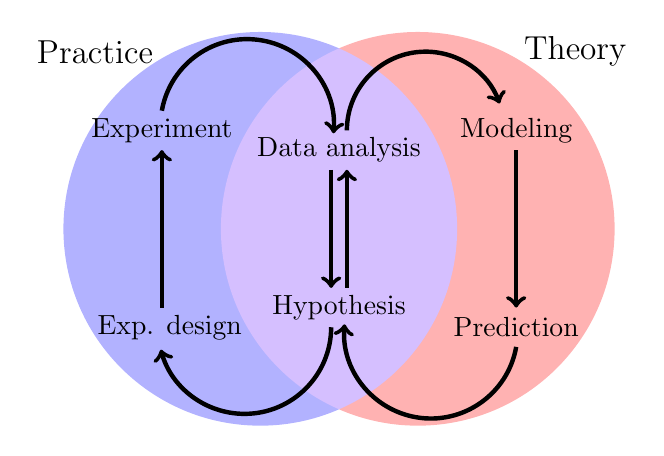
\begin{tikzpicture}
			\pgftransformscale{\myscalefactor}
			\begin{scope}[blend group = soft light]
				\fill[blue!30!white] (-2,0) ellipse (5 and 5);
				\fill[red!30!white]  (+2,0) ellipse (5 and 5);
			\end{scope}
			\draw[ultra thick, ->] (0.2,2.5) arc (0:-160:-2);
			\draw[ultra thick, ->] (-4.5,+3) arc (-10:-185:-2.2);
			\draw[ultra thick, ->] (-0.2,-2.5) arc (0:-165:+2.2);
			\draw[ultra thick, ->] (4.5,-3) arc (-10:-185:2.2);
			\draw [ultra thick, ->] (-0.2,+1.5) -- (-0.2,-1.5);
			\draw [ultra thick, ->] (+0.2,-1.5) -- (+0.2,+1.5);
			\draw [ultra thick, ->] (4.5,+2) -- (4.5,-2);
			\draw [ultra thick, ->] (-4.5,-2) -- (-4.5,+2);
			\node at (0,+2) {Data analysis};
			\node at (4.5,+2.5)  {Modeling};
			\node at (4.5,-2.5)  {Prediction};
			\node at (0,-2)  {Hypothesis};
			\node at (-4.5,+2.5)  {Experiment};
			\node at (-4.3,-2.5) {Exp. design};
			\node at (-6.2,4.5)[font=\large]    {Practice};
			\node at (+6,4.5)[font=\large]    {Theory};
		\end{tikzpicture}
	\\ \vspace{0.5cm}
	\small
	Practice and theory in engineering and scientific research. The focus is to use modeling to make predictions outside previous experimental settings to come of with a better control/decision. 
\end{frame}

%-------------------------------------------------%
\section{Chemotherapy}

\begin{frame}{Cyclophosphamide: innate immune cell recruitment and tumor regression}
	The current standard of care limits the regimens used primarily to daily dose and maximum-tolerated dose (MTD) treatments.
	\vspace{1cm}
	\begin{itemize}
		\item Motivation: Metronomic/intermittent experiments~\footfullcite{wu2014metronomic} in mice. A lower dose with a higher frequency than MTD was shown to recruit the immune system and reduce the tumor volume.
		\vspace{0.5cm}
		\item Objective: Use optimal control techniques in order to have a better treatment outcome among all possible dosing strategies.
	\end{itemize}
\end{frame}

\begin{frame}{Optimal control techniques for cancer treatment}
	Early efforts in using optimal control techniques for cancer treatment started in the 1970s for Radiotherapy~\footfullcite{bahrami1975optimal} and Chemotherapy~\footfullcite{swan1977optimal} treatments. \\
	\vspace{0.5cm}
	A new generation of quantitative experiments made it possible to have more realistic models of the system. \\
	\vspace{0.5cm}
	The goal is to use optimal control techniques to find a mathematically derived optimal regimen (MDOR) to be tested in similar experimental settings.
\end{frame}

\subsection{Model}
\begin{frame}{A dynamic model for chemotherapy}
	\small
	Model is fitted to the tumor and immune data in mouse experiments.\\
	\begin{subequations} \label{eq:chemo1}
		\begin{align} 
			\dot{T}(t) &=  k_{a} T(t) - \frac{k_{b}C(t)T(t)}{k_{c}C(t)+T(t)} - k_{d}T(t)I(t),\\
			\dot{I}(t) &= q X(t) -k_{e}T(t)I(t)-k_{f}C(t)I(t)-k_{g}Y(t)I(t)-k_{h}I(t),\\
			\dot{X}(t) &= \frac{q C(t)T(t)}{k_{i}C(t)+T(t)}-k_{j}X(t)-k_{k}X(t)Y(t),\\
			\dot{Y}(t) &= \frac{I(t)}{k_l+I(t)} - k_{m}Y(t) C(t),\\
			\dot{C}(t) &= u(t) - \frac{k_1 C(t)}{k_2 + C(t)}.
		\end{align}
	\end{subequations} \\ 
	$T$:tumor volume. Variables $I$:immune system, $X$:immunostimulatory, $Y$:immunossuppressor, and $C$:drug are phenamenological. 
\end{frame}

%\begin{frame}{Steady-states of the model}
%	
%\end{frame}

\subsection{Metronomic}
\begin{frame}{Efficacy of metronomic regimens}
	140 mg/kg every 6 days as an optimal metronomic regimen. \\ \vspace{0.5cm}
	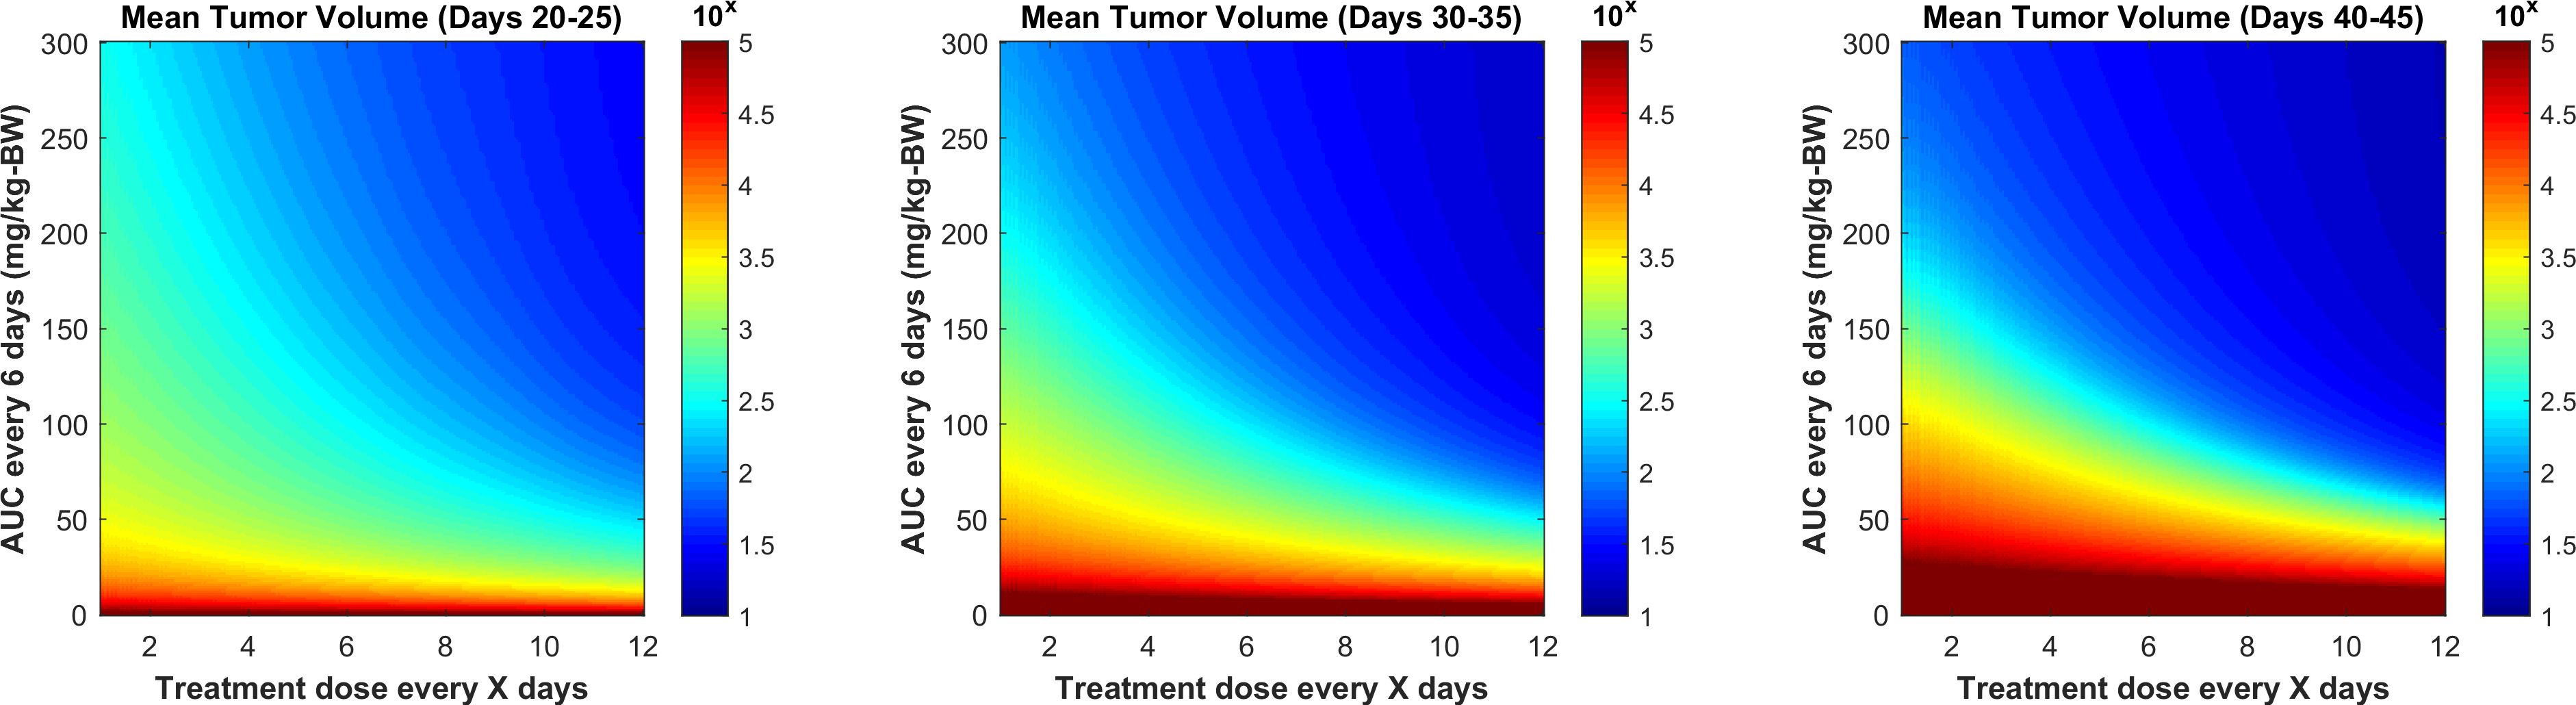
\includegraphics[width=1\linewidth]{chemo-metronomic.png} \\
	\vspace{0.5cm}
	The average tumor volume at different time ranges of 20-25 days (left), 30-35 days (middle), and 40-45 days (right) after starting metronomic regimens. The horizontal axis represents the number of days between each dose, y-axis is the total amount of drug given to the animal every 6 days.
\end{frame}

\subsection{Optimal control}
\begin{frame}{Optimal control problem setup}
	Numerical software GPOPS\textunderscore II is used to solve the following setup of optimal control problem.\\
	\begin{subequations}
	\begin{align}  \label{eq:ocp}
			\min_{u(t)} & \quad T(t_f), \\
			s.t. & \quad 
			\begin{bmatrix}
				0 \\ 0 \\ 0 \\ 0 \\ 0 \\ 0
			\end{bmatrix} 
			\leq
			\begin{bmatrix}
				C(t) \\ T(t) \\ I(t) \\ X(t) \\ Y(t) \\ u(t)
			\end{bmatrix}
			\leq
			\begin{bmatrix}
				C_m \\ T_m \\ I_m \\ X_m \\ Y_m \\ u_m
			\end{bmatrix},
			\\
			& \quad \int_0^{t_f} u(t) dt \leq U_m.
	\end{align}
	\end{subequations}
\end{frame}

\begin{frame}{Numerical result for a low input upper bound}
	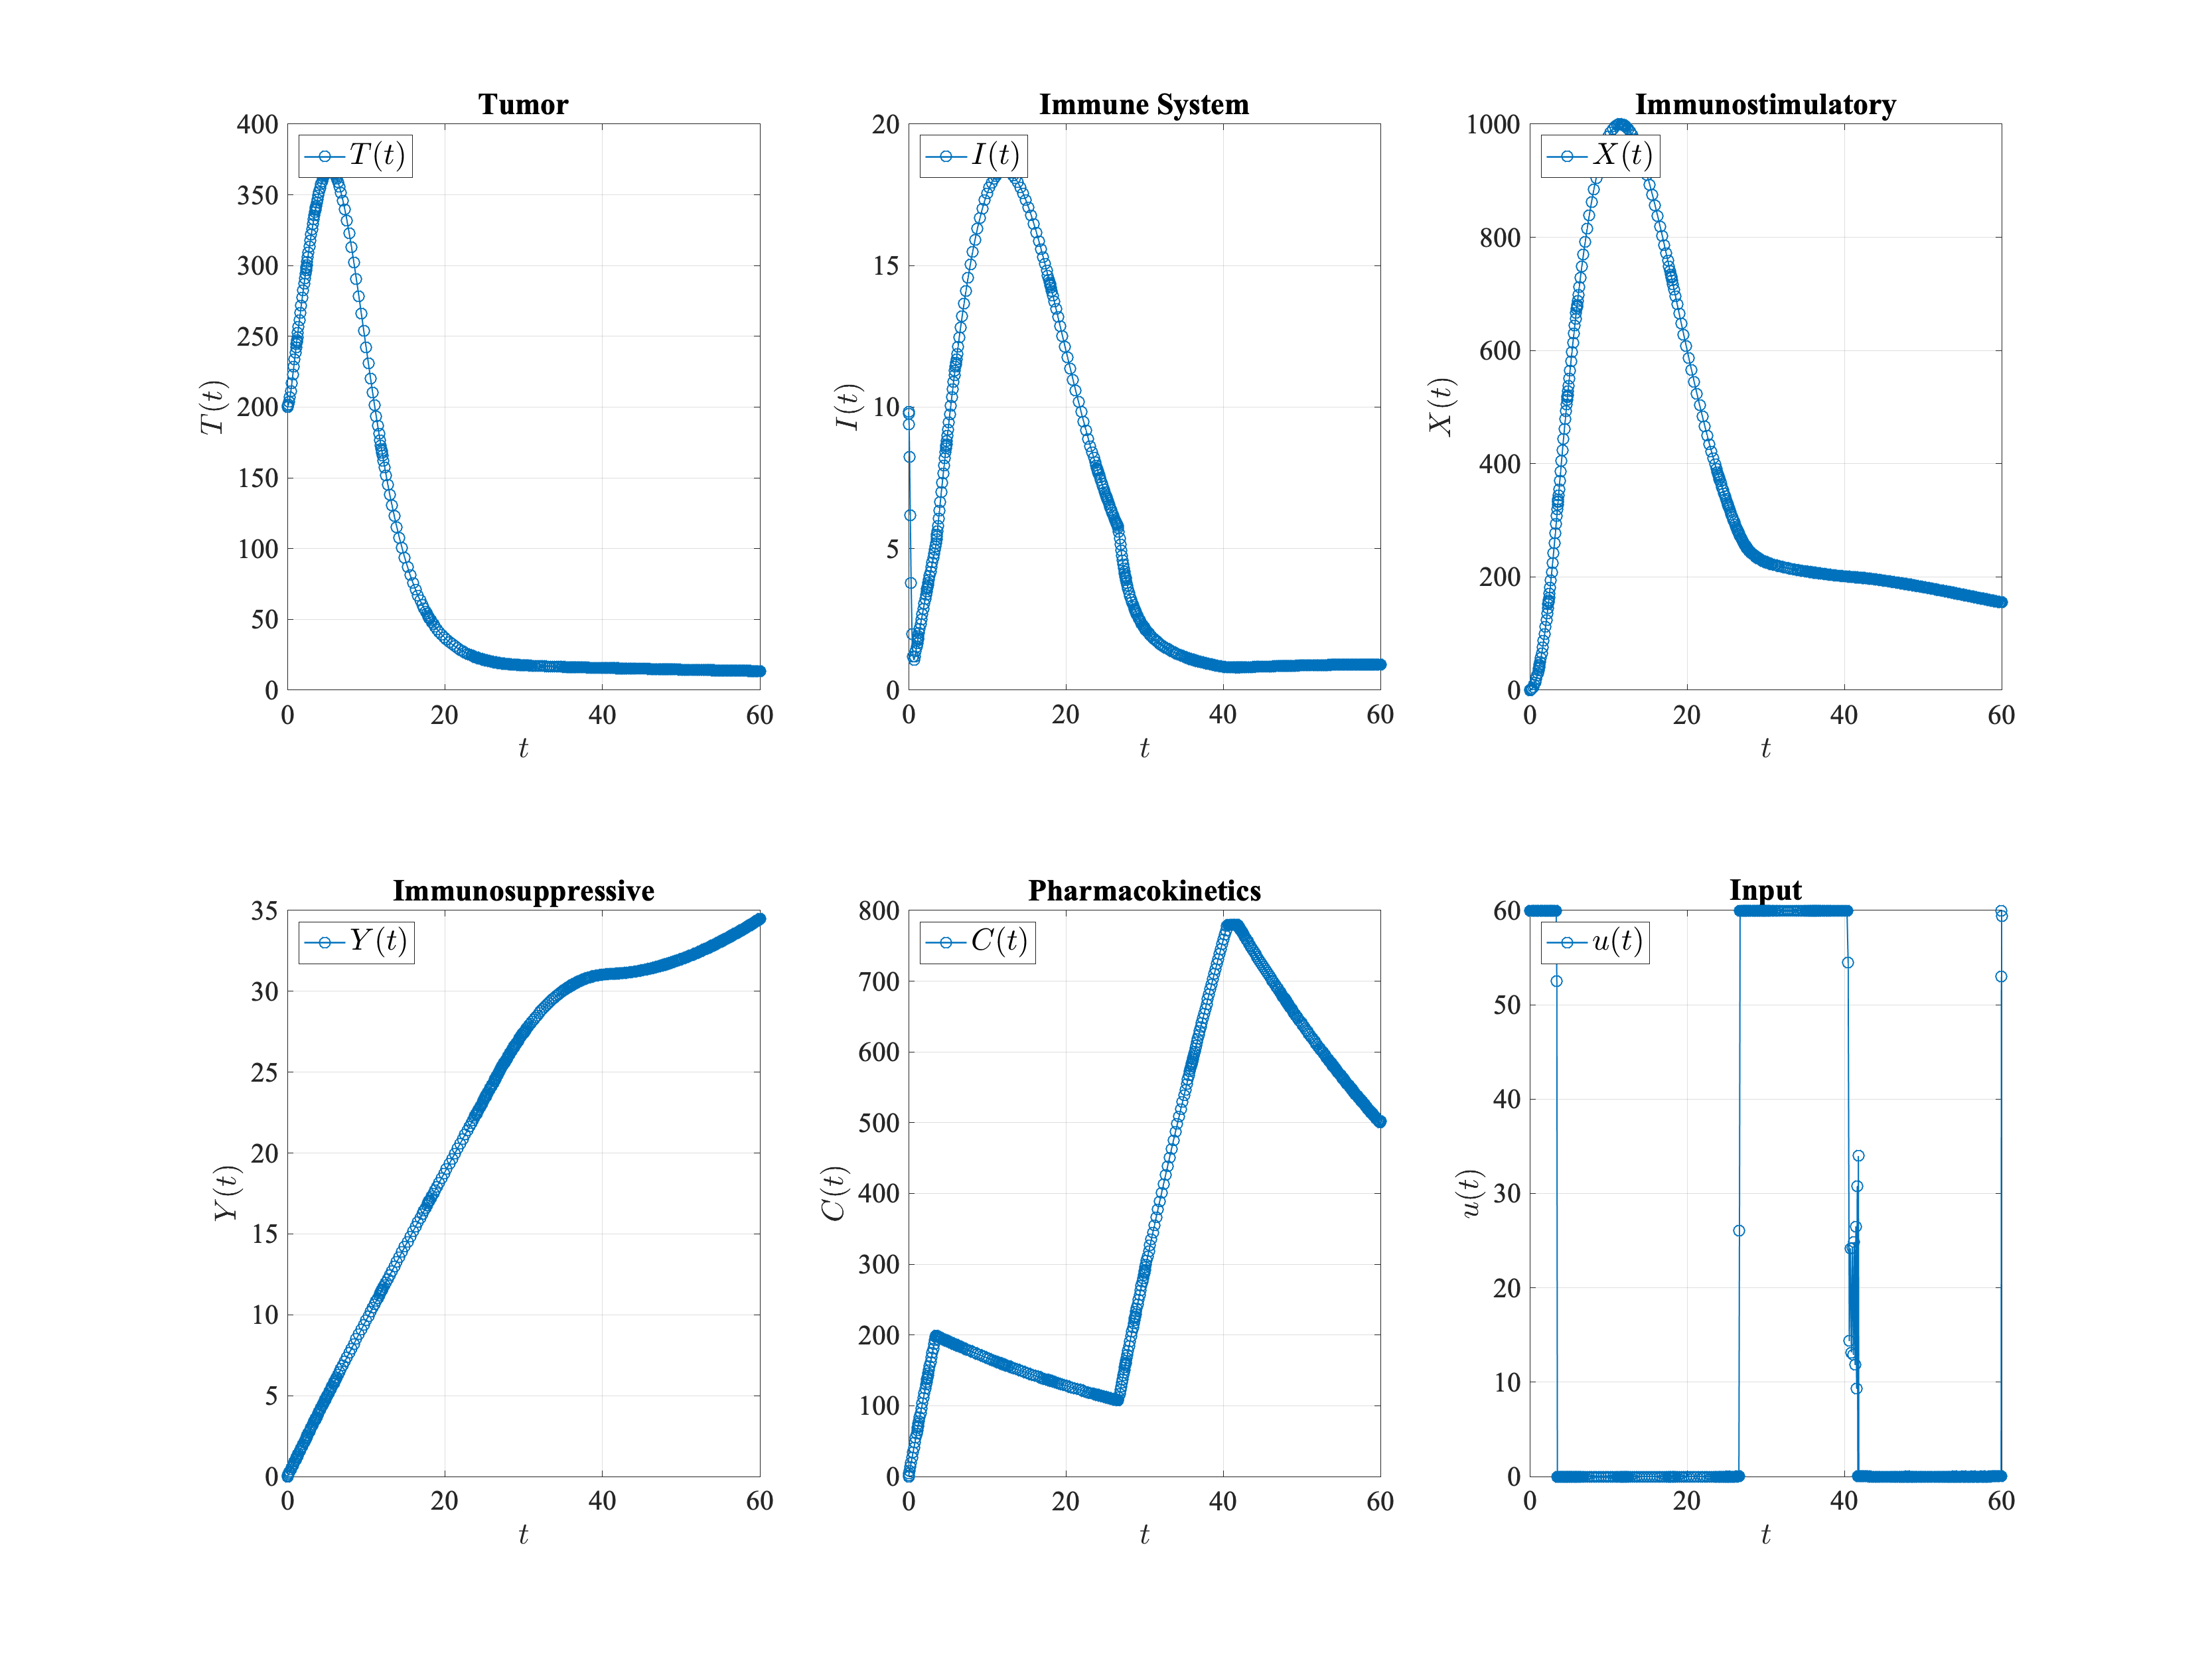
\includegraphics[width=1\linewidth]{chemo-optimalcontrol1.png} \\
	Circles show the final collocation points.
\end{frame}

\begin{frame}{Numerical result for a high input upper bound}
	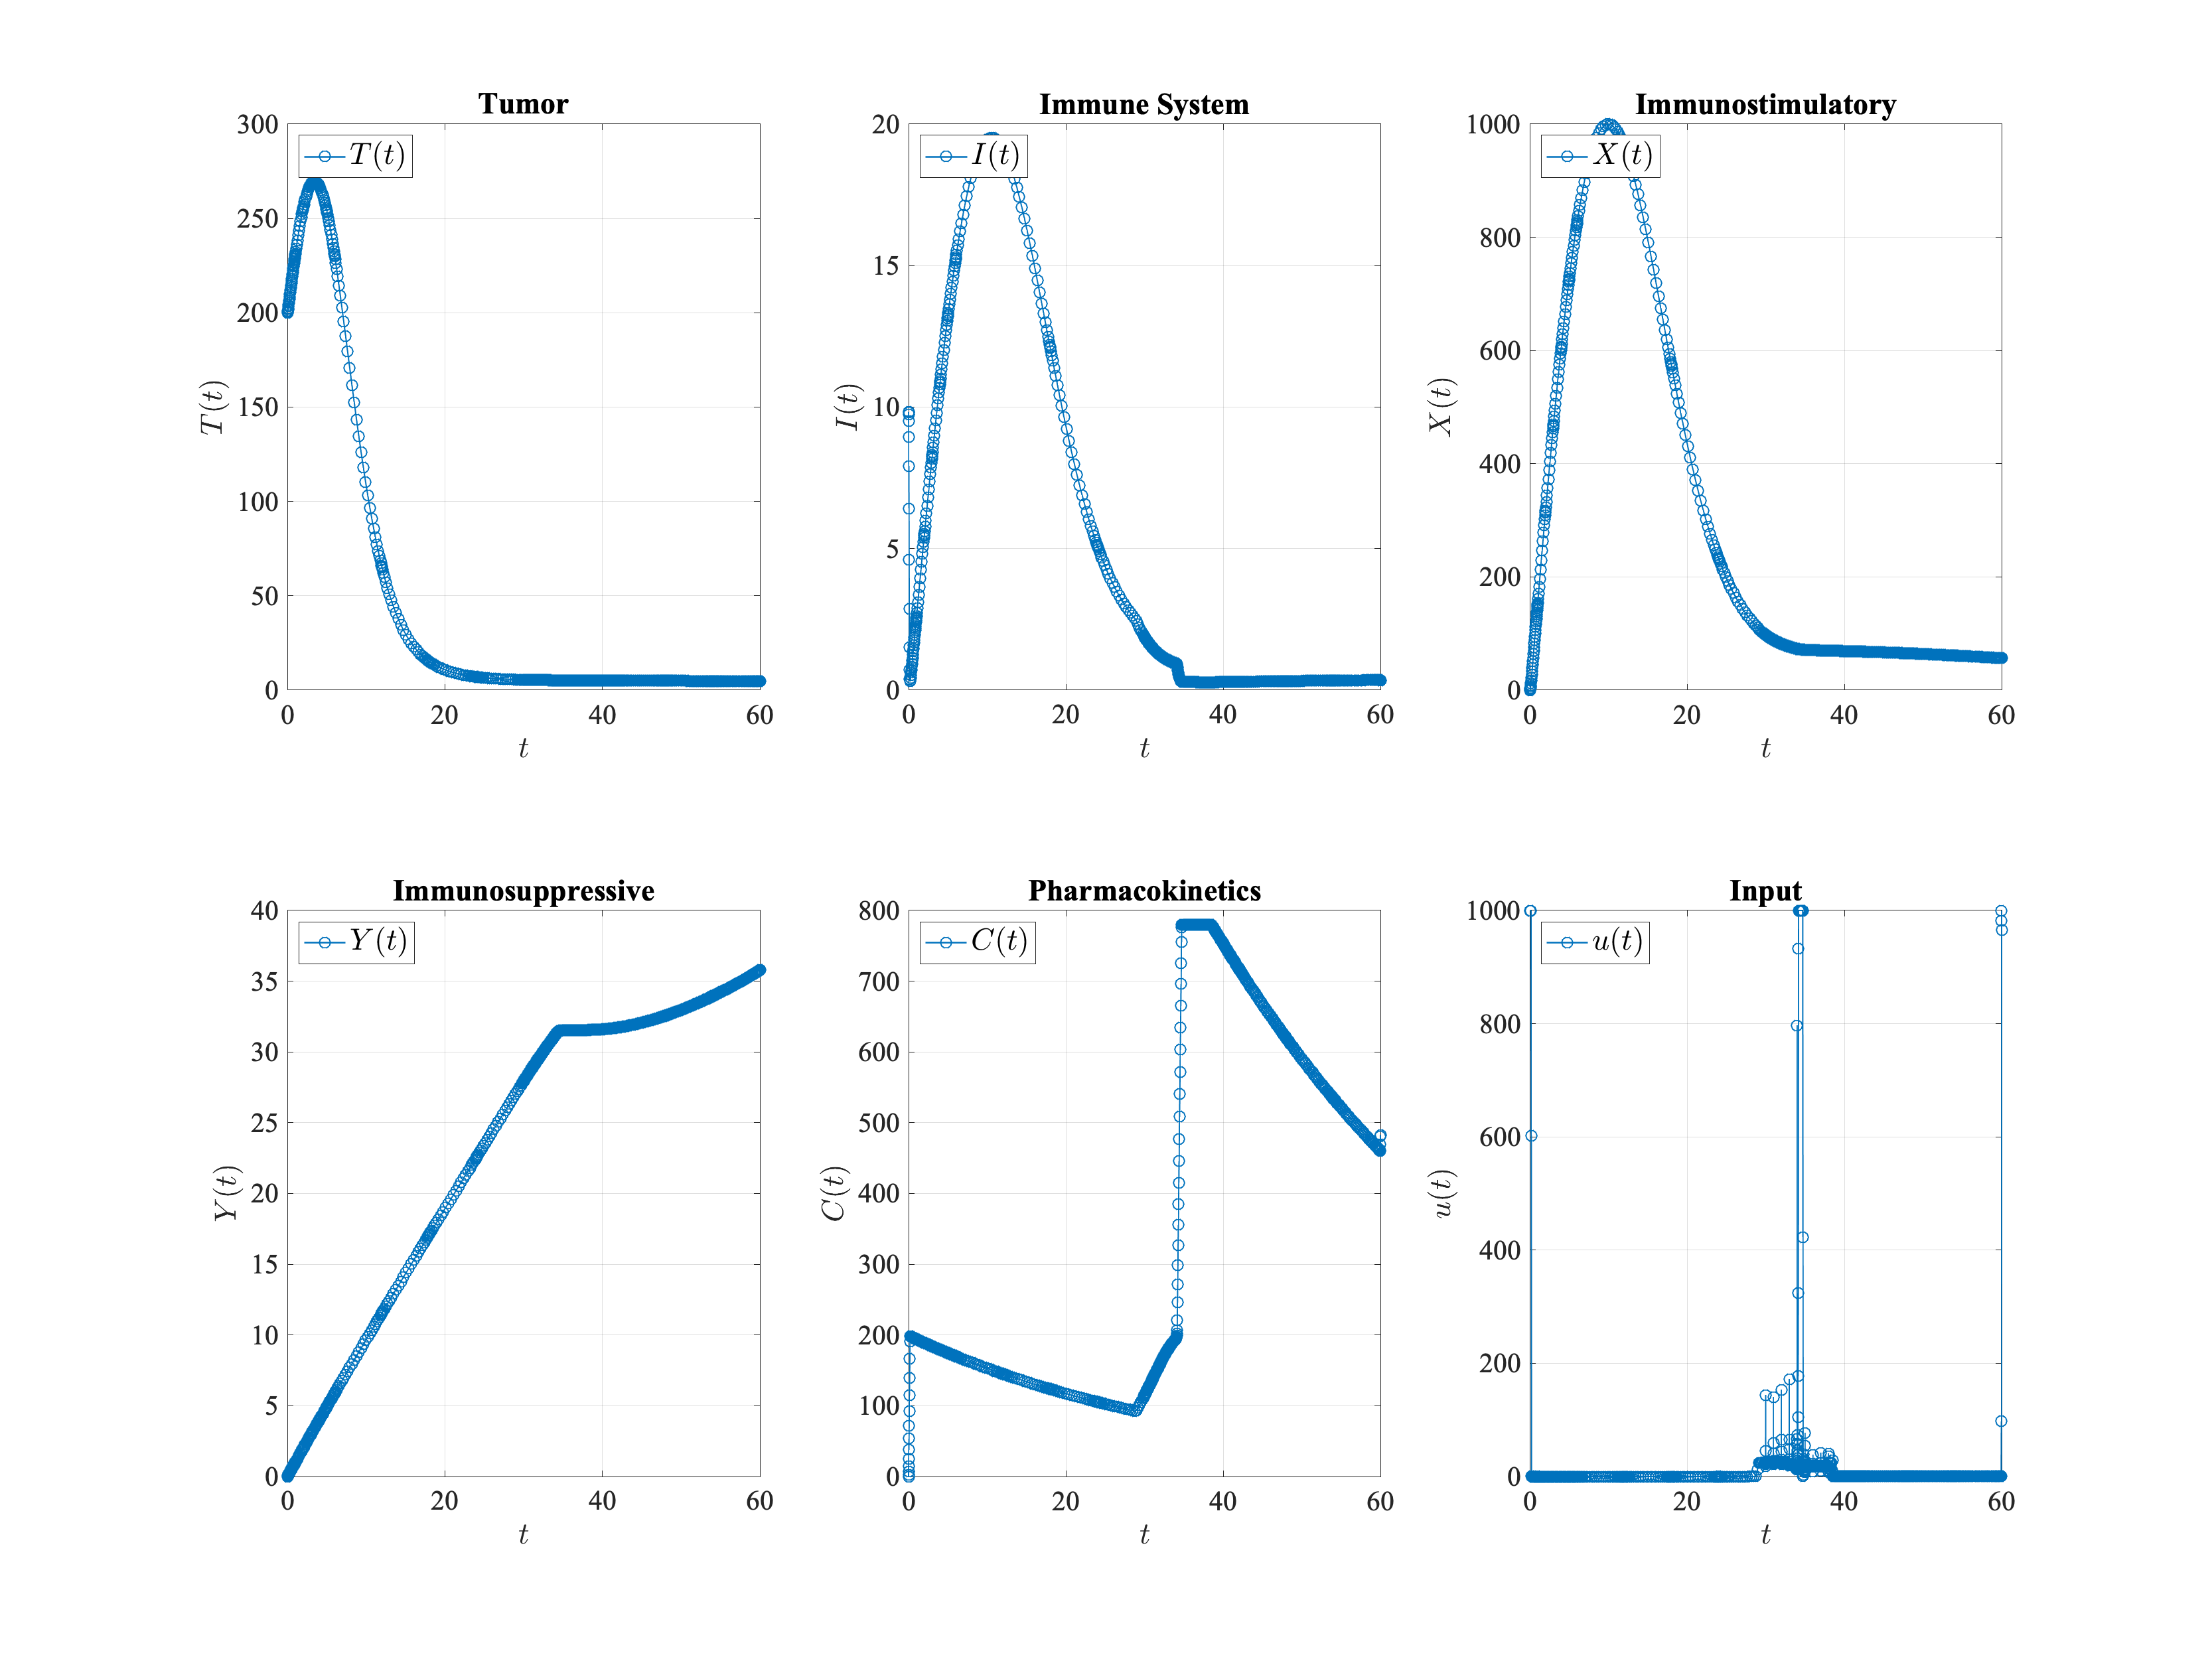
\includegraphics[width=1\linewidth]{chemo-optimalcontrol2.png} \\
	Circles show the final collocation points.
\end{frame}

\subsection{MDOR}
\begin{frame}{Optimal control vs. metronomic regimen}
	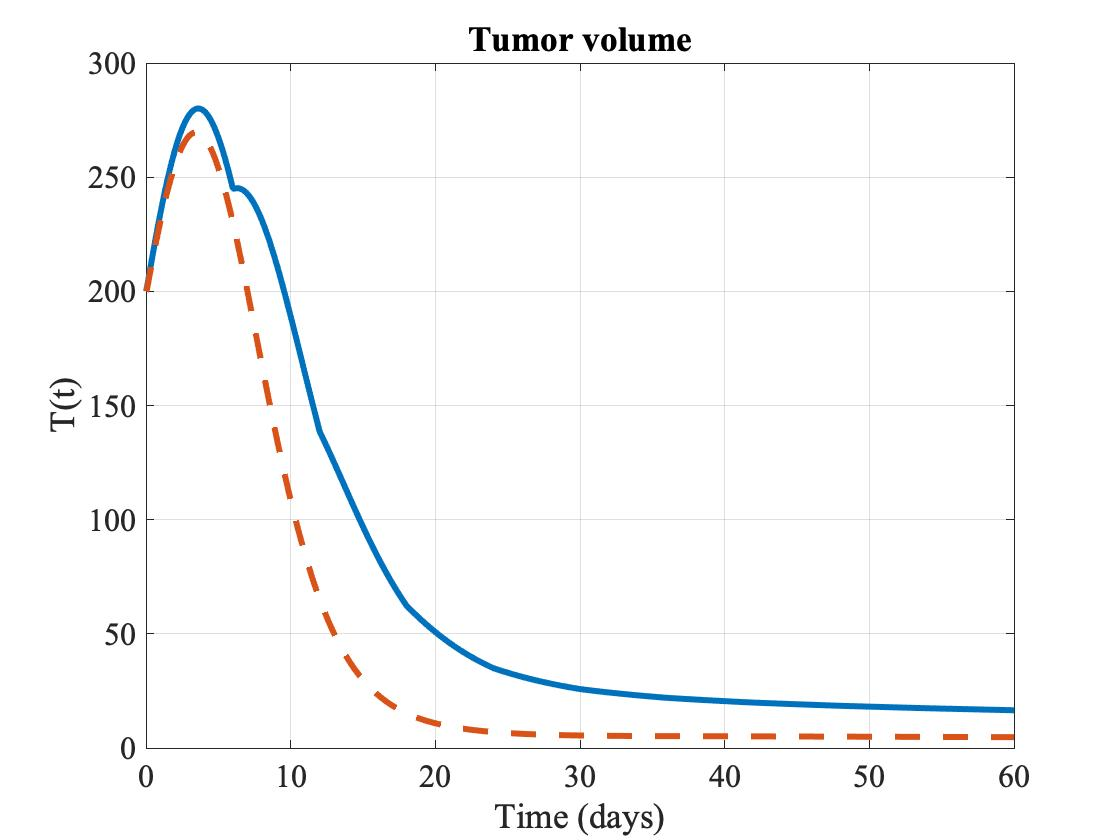
\includegraphics[width=0.49\textwidth]{chemo-comparison-oc1.jpeg}
	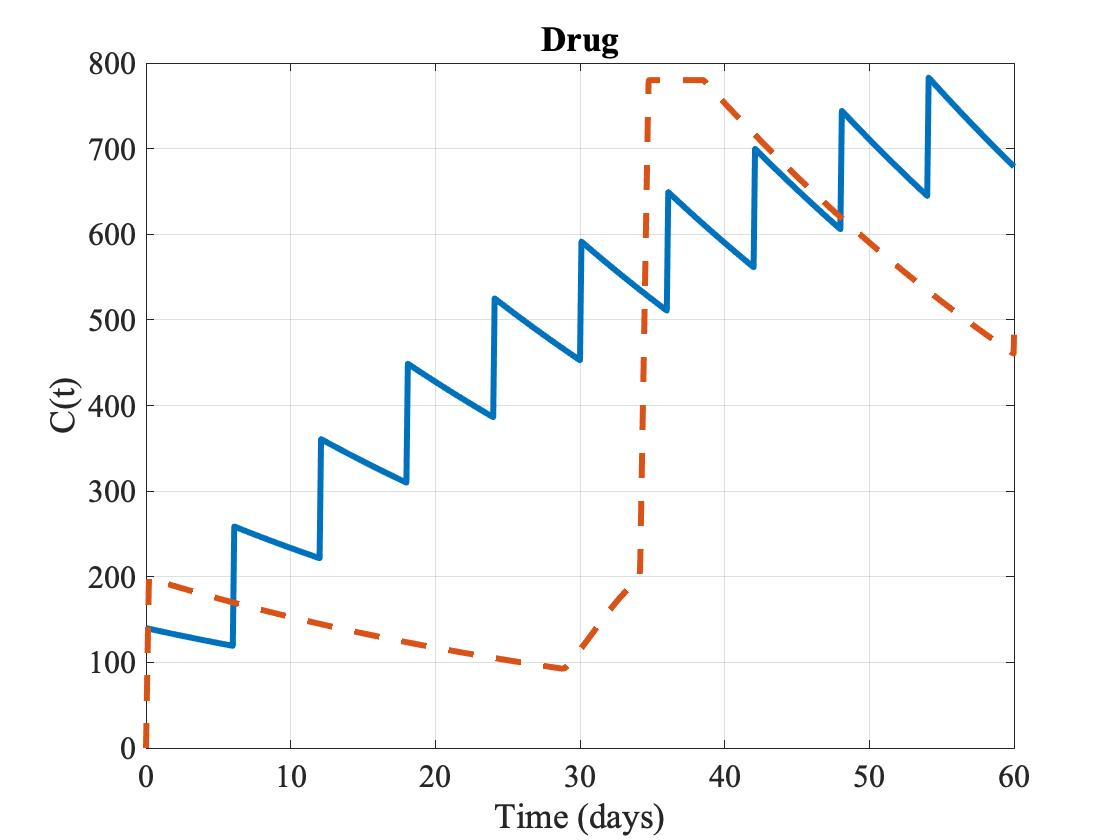
\includegraphics[width=0.49\textwidth]{chemo-comparison-oc2.jpeg} \\
	Comparing a standard 140 mg/kg Q6D metronomic chemotherapy plan (solid lines) with the obtained optimal control (dashed lines). \\ \vspace{0.5cm}
	The numerical results can be interpreted as two-dose of 200mg/kg and 600mg/kg regimen. However, the maximum tolerated dose is 300mg/kg/day for the chemotherapy drug.
\end{frame}

\begin{frame}{Mathematically derived optimal regimen}
	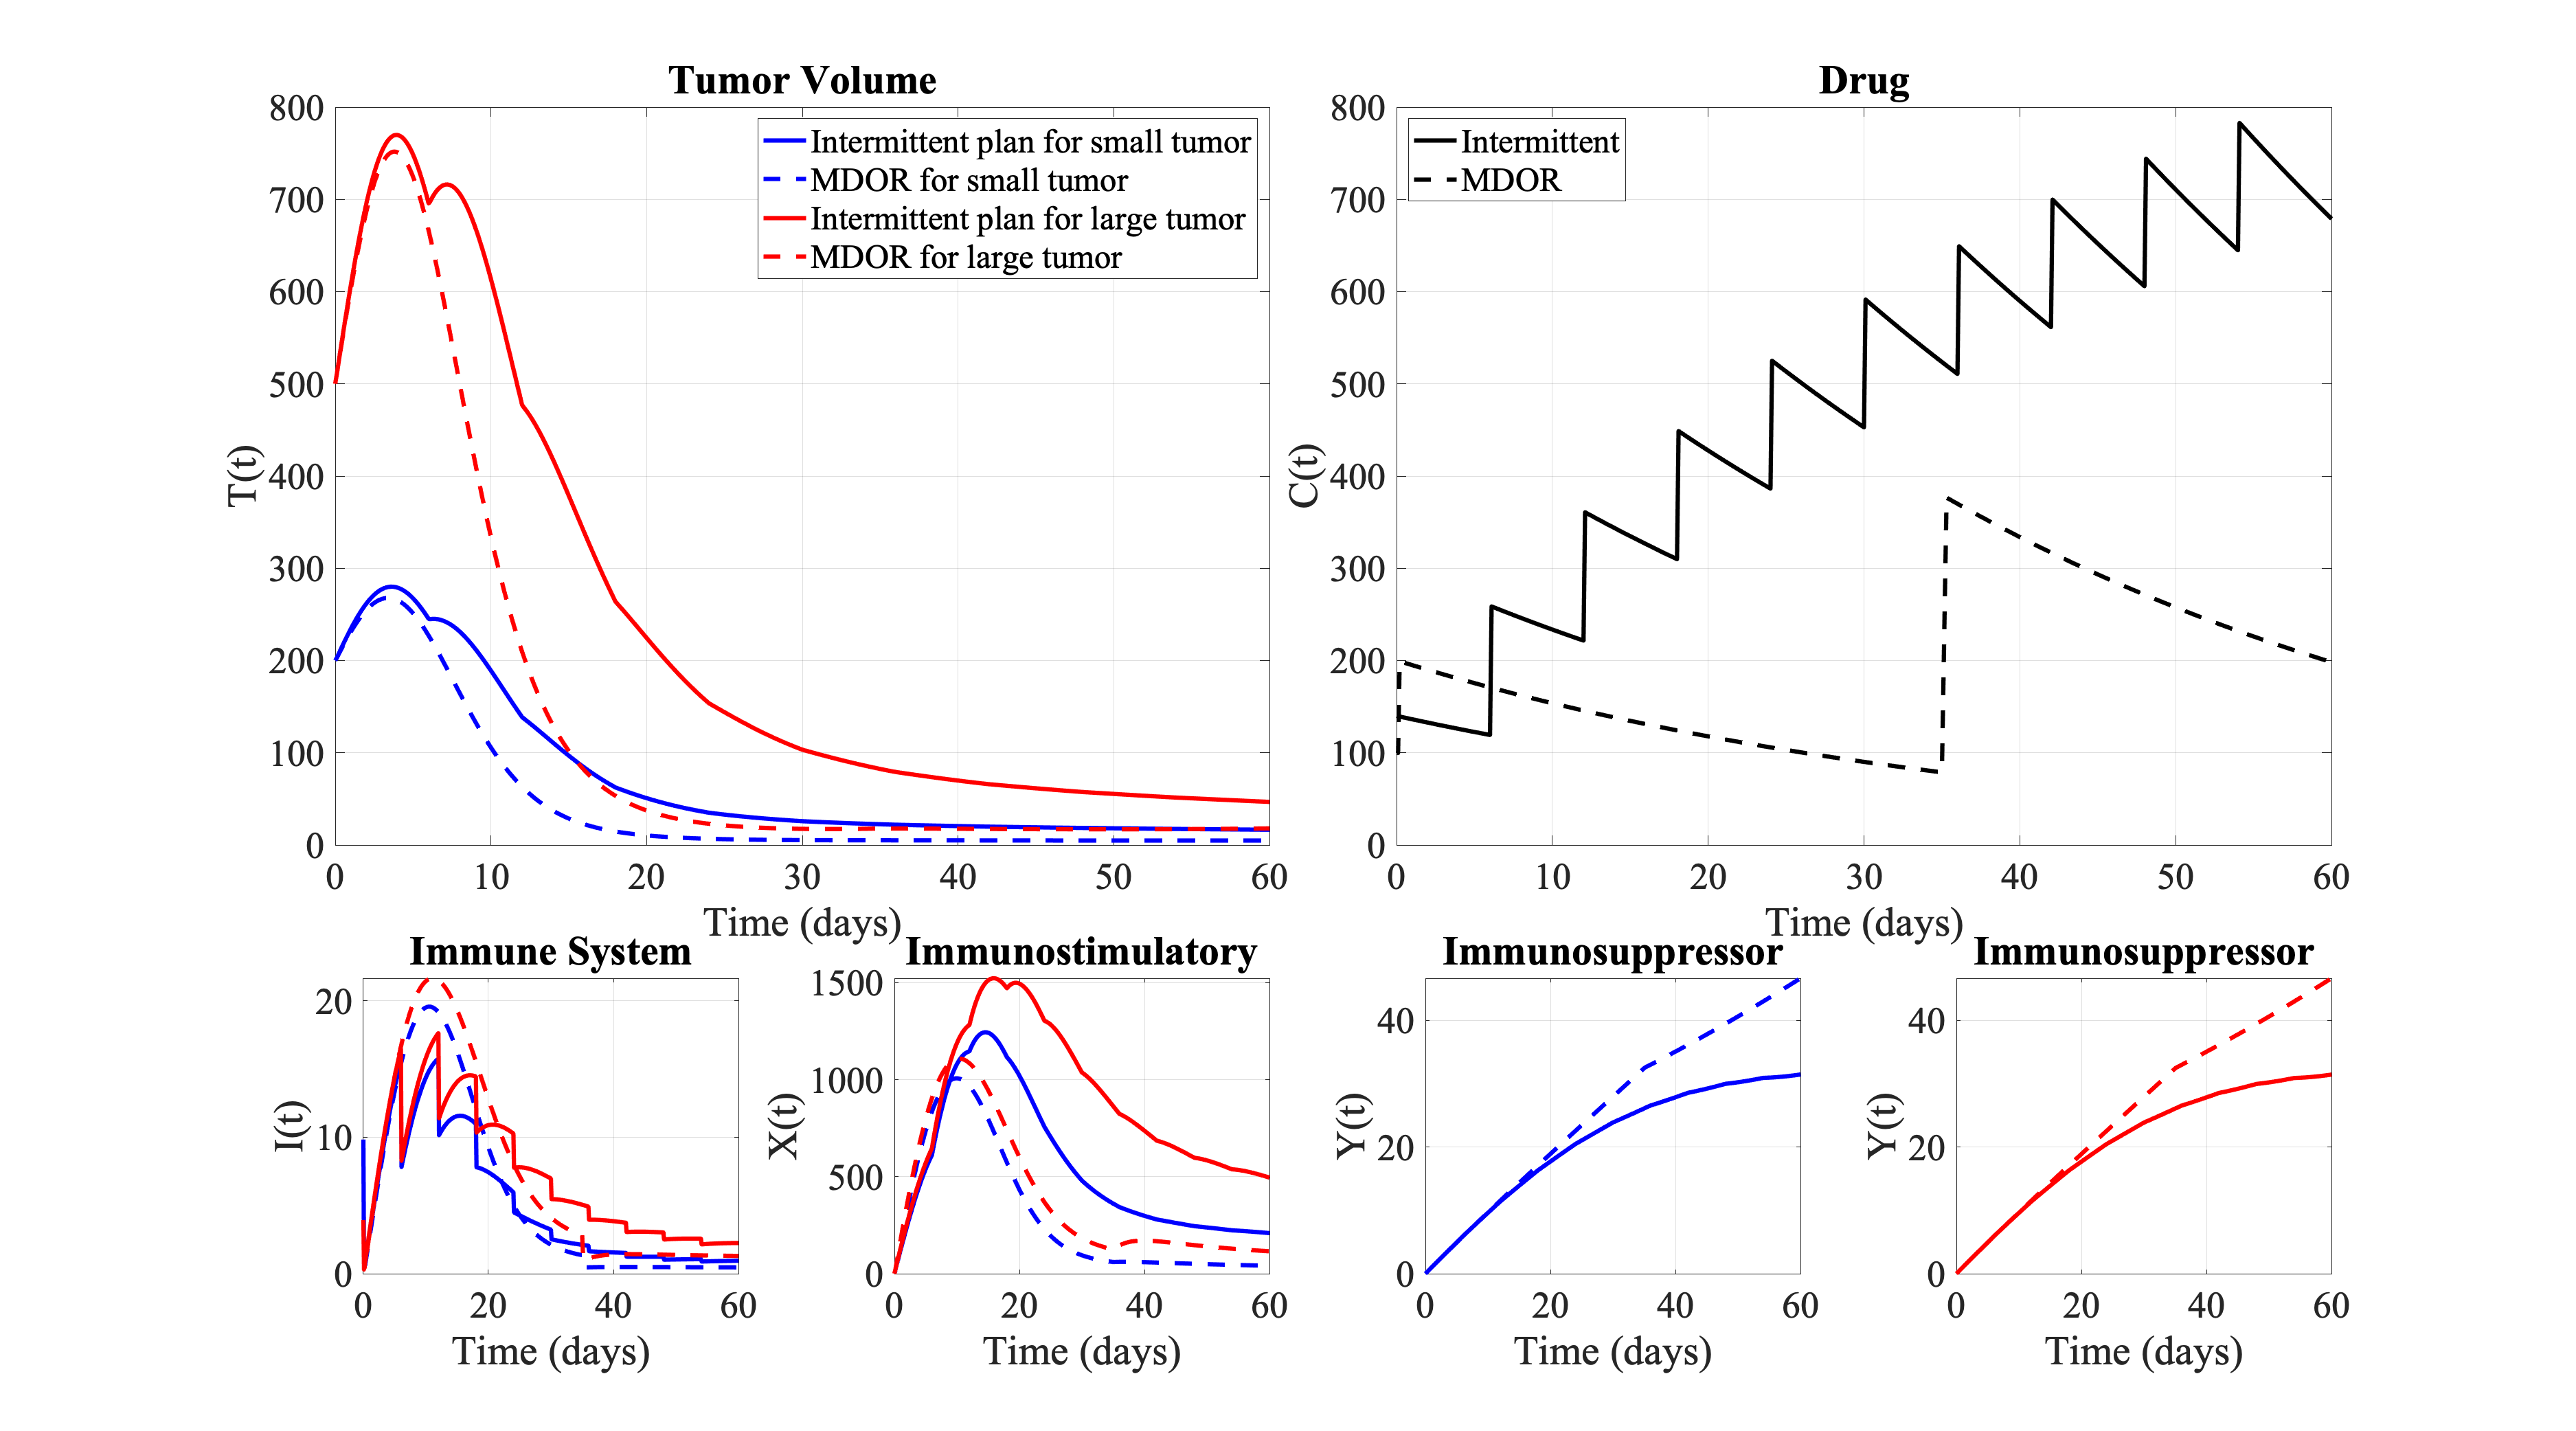
\includegraphics[width=1\textwidth]{chemo-final.png} \\
	Comparing a standard 140 mg/kg Q6D metronomic/intermittent plan (solid lines) and the mathematically derived optimal regimen (dashed lines). 
\end{frame}

\begin{frame}{A new viable regimen to be tested experimentally}
	\hspace{1cm}
	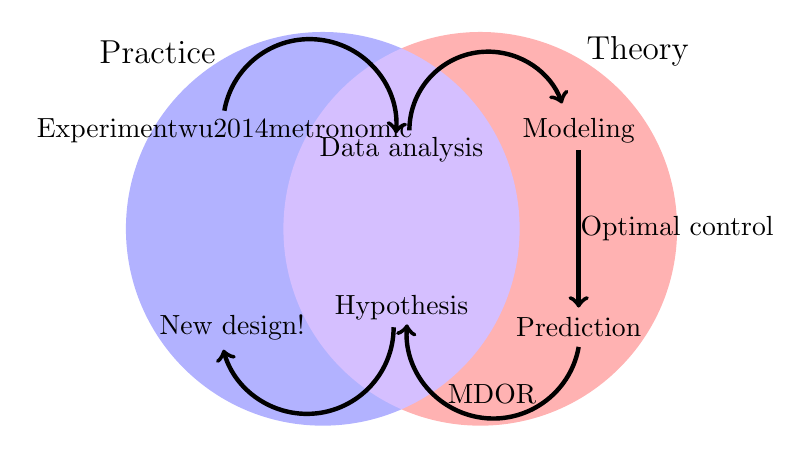
\begin{tikzpicture}
		\pgftransformscale{\myscalefactor}
		\begin{scope}[blend group = soft light]
			\fill[blue!30!white] (-2,0) ellipse (5 and 5);
			\fill[red!30!white]  (+2,0) ellipse (5 and 5);
		\end{scope}
		\draw[ultra thick, ->] (0.2,2.5) arc (0:-160:-2);
		\draw[ultra thick, ->] (-4.5,+3) arc (-10:-185:-2.2);
		\draw[ultra thick, ->] (-0.2,-2.5) arc (0:-165:+2.2);
		\draw[ultra thick, ->] (4.5,-3) arc (-10:-185:2.2);
%		\draw [ultra thick, ->] (-0.2,+1.5) -- (-0.2,-1.5);
%		\draw [ultra thick, ->] (+0.2,-1.5) -- (+0.2,+1.5);
		\draw [ultra thick, ->] (4.5,+2) -- (4.5,-2);
%		\draw [ultra thick, ->] (-4.5,-2) -- (-4.5,+2);
		\node at (0,+2) {Data analysis};
		\node at (4.5,+2.5)  {Modeling};
		\node at (7,+0.0)  {Optimal control};
		\node at (2.3,-4.2)  {MDOR};
		\node at (4.5,-2.5)  {Prediction};
		\node at (0,-2)  {Hypothesis};
		\node at (-4.5,+2.5)  {Experiment\footfullcite{wu2014metronomic}};
		\node at (-4.3,-2.5) {New design!};
		\node at (-6.2,4.5)[font=\large]    {Practice};
		\node at (+6,4.5)[font=\large]    {Theory};
	\end{tikzpicture}
\end{frame}

%-------------------------------------------------%
\section{Epidemic}

\begin{frame}{Social distancing (SD) in epidemics}
	During the COVID-19 epidemic, social distancing as a form of non-pharmaceutical intervention has been enacted in the US and other countries.
	\vspace{1cm}
	\begin{itemize}
		\item Motivation: Shortening the period of time that populations are socially distanced is economically advantageous.  
		\vspace{0.5cm}
		\item Objective: To reduce the disease burden (here measured as the peak of the infected population) while simultaneously minimizing the length of time that the population is socially distanced.  
	\end{itemize}
\end{frame}

\subsection{Singel interval SD}

\begin{frame}{Early days and limited data}
	\vspace{0.5cm}
	\hspace{1cm}
	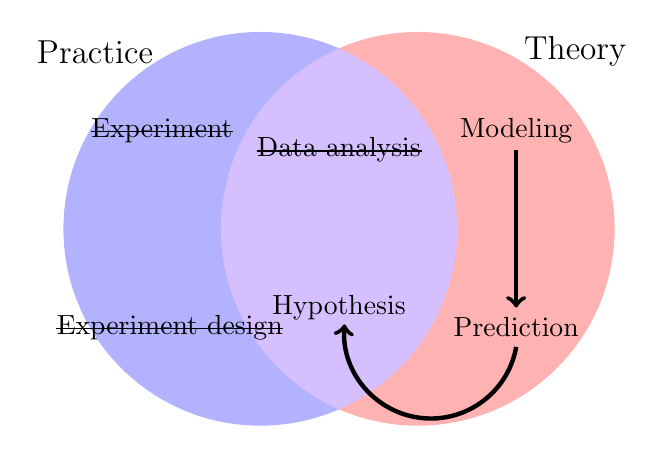
\begin{tikzpicture}
		\pgftransformscale{\myscalefactor}
		\begin{scope}[blend group = soft light]
			\fill[blue!30!white] (-2,0) ellipse (5 and 5);
			\fill[red!30!white]  (+2,0) ellipse (5 and 5);
		\end{scope}
		%		\draw[ultra thick, ->] (0.2,2.5) arc (0:-160:-2);
		%		\draw[ultra thick, ->] (-4.5,+3) arc (-10:-185:-2.2);
		%		\draw[ultra thick, ->] (-0.2,-2.5) arc (0:-165:+2.2);
		\draw[ultra thick, ->] (4.5,-3) arc (-10:-185:2.2);
		%		\draw [ultra thick, ->] (-0.2,+1.5) -- (-0.2,-1.5);
		%		\draw [ultra thick, ->] (+0.2,-1.5) -- (+0.2,+1.5);
		\draw [ultra thick, ->] (4.5,+2) -- (4.5,-2);
		%		\draw [ultra thick, ->] (-4.5,-2) -- (-4.5,+2);
		\node at (0,+2) {\st{Data analysis}};
		\node at (4.5,+2.5)  {Modeling};
		\node at (4.5,-2.5)  {Prediction};
		\node at (0,-2)  {Hypothesis};
		\node at (-4.5,+2.5)  {\st{Experiment}};
		\node at (-4.3,-2.5) {\st{Experiment design}};
		\node at (-6.2,4.5)[font=\large]    {Practice};
		\node at (+6,4.5)[font=\large]    {Theory};
	\end{tikzpicture}
\end{frame}

\begin{frame}{Mathematical model for a single interval SD}
	Assuming that $\beta$, the disease transmission rate, can be effectively reduced from $\beta_{n}$ (contact rate during normal time for non-distanced population) to $\beta_{d}$ (contact rate during social distancing) during distancing. \\ \vspace{0.5cm}
	\begin{equation} \label{eq:beta}
		\beta(t) = \left\{
		\begin{matrix} 
			\beta_n & \qquad 0 \leq t_s \\ 
			\beta_d & \qquad t_s \leq t < t_s+t_d \\
			\beta_n  & \qquad t_s+t_d \leq t 
		\end{matrix}
		\right. .
	\end{equation} \\ \vspace{0.5cm}
	Normalized infected population in \textit{SIR} model, with no re-infection. \\
	\hspace{2cm} 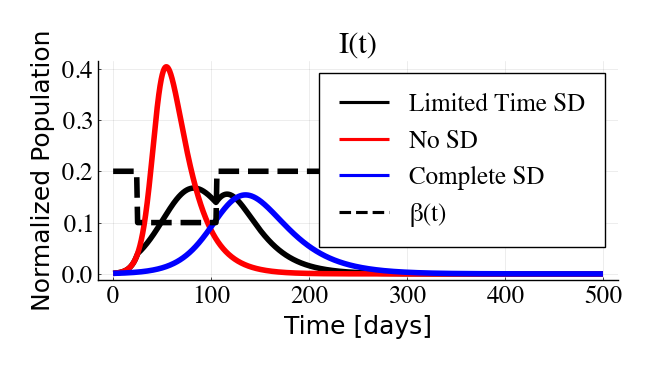
\includegraphics[width=0.6\textwidth]{epidemic-sd.png}\\
\end{frame}

\begin{frame}{Optimize start time $t_s$ and duration $t_d$ of SD}
	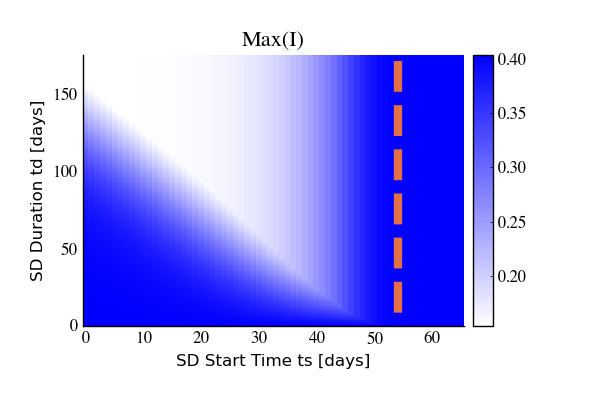
\includegraphics[width=0.49\textwidth]{epidemic-sir-heatmap.png}
	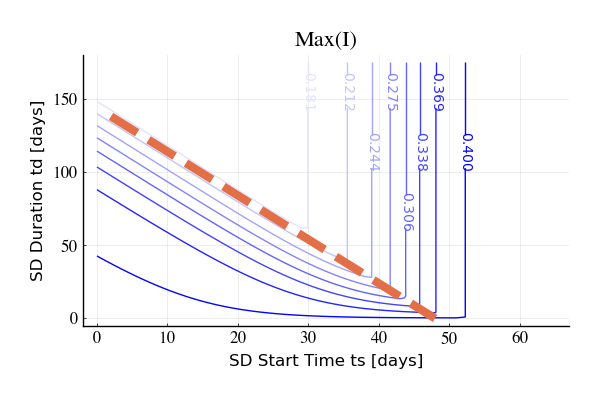
\includegraphics[width=0.49\textwidth]{epidemic-sir-contour.png} \\ \vspace{0.5cm}
	Infected peak, $\mbox{Max}(I)$, in \textit{SIR} model under single interval SD policy. The vertical dashed line represents the time of infected peak for a normal population with no distancing. The diagonal dashed line represents an analytically derived slope approximation.
\end{frame}

\begin{frame}{A common ``V'' shape pattern}
	Each model is simulated with parameters in the respective papers and assumed to be appropriate, based on data available at the time, for the COVID-19 pandemic.\\  \vspace{0.5cm}
	\hspace{1cm}  \textit{SIR} \hspace{2.5cm} \textit{SAIR} \hspace{2.1cm} \textit{f-SIR} \\
	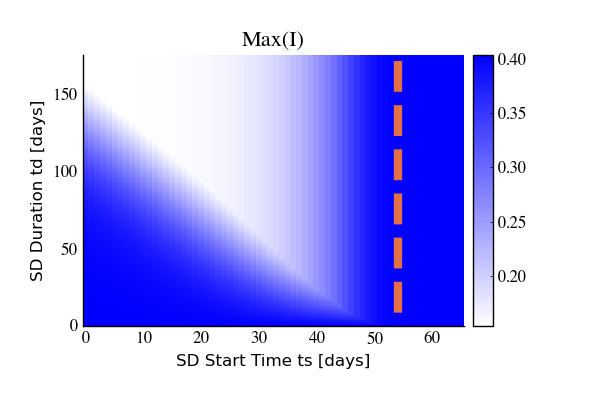
\includegraphics[width=0.32\textwidth]{epidemic-sir-heatmap.png}
	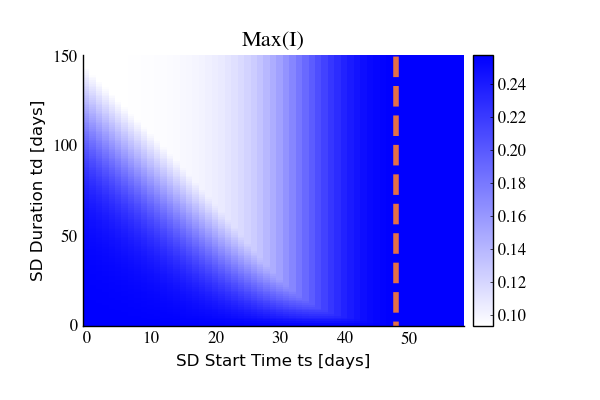
\includegraphics[width=0.32\textwidth]{epidemic-sair.png}
	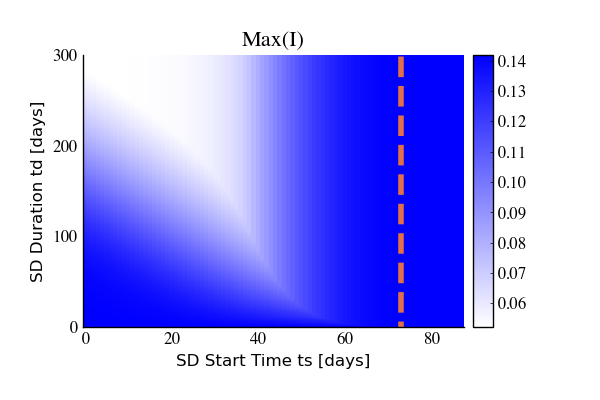
\includegraphics[width=0.32\textwidth]{epidemic-fsir.png}\\
	\hspace{0.8cm}  \textit{6-SIR} \hspace{2.3cm} \textit{SIQR} \hspace{1.8cm} \textit{SIDARTHE} \\
	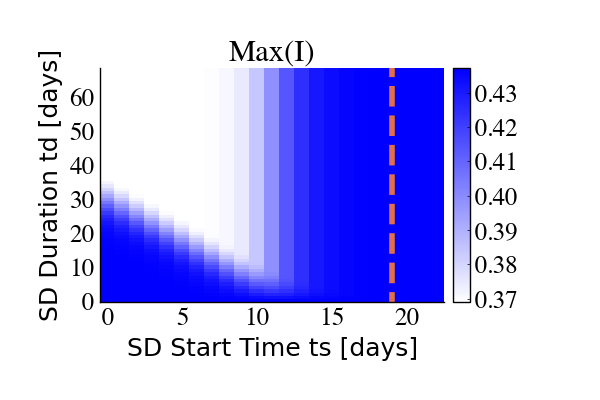
\includegraphics[width=0.32\textwidth]{epidemic-sixsir.png}
	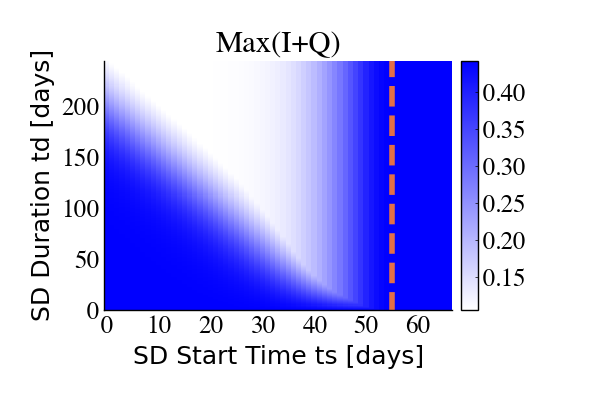
\includegraphics[width=0.32\textwidth]{epidemic-siqr.png}
	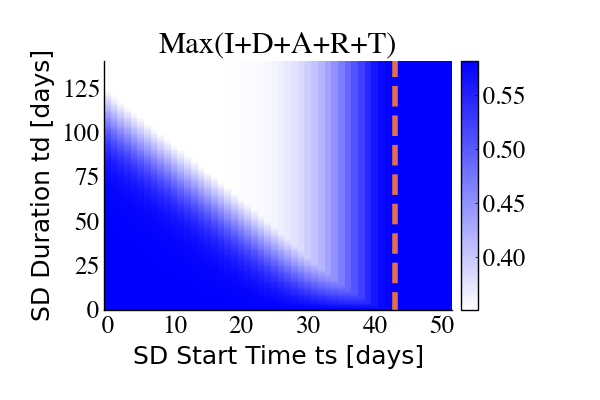
\includegraphics[width=0.32\textwidth]{epidemic-sidarthe.png}
\end{frame}

\subsection{Periodic SD}
\begin{frame}{Periodic relaxation is economically favorable}
	 A policy with regular periods of distancing and relaxation can significantly delay the time of the peak of the epidemic, while still allowing limited economic activity. \\ \vspace{1cm}
	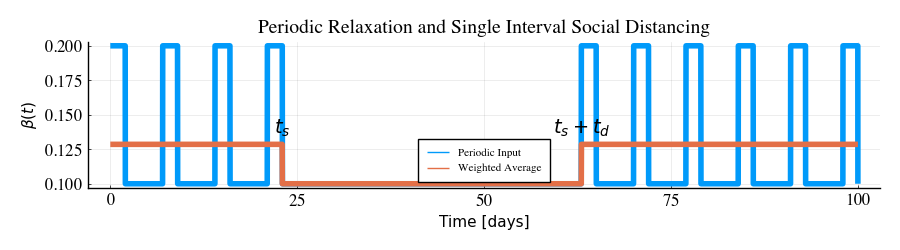
\includegraphics[width=1\textwidth]{epidemic-combination.png}
\end{frame}

\begin{frame}{Periodic relaxation and non-monotonicity}
	The peak of infected population depends non-monotonically on both the period $T$ and ratio $r$ of periodic policies. \\ \vspace{0.5cm}
	A periodic social distancing relaxation policy with a large period time $T$ may lead to high transmission rates at the critical time of an epidemic (e.g. at the potential peak of the infected population).  \\ \vspace{0.5cm}
	Or it may lead to a well-timed strategy and hence significantly reduce the infected peak. \\ \vspace{0.5cm}
	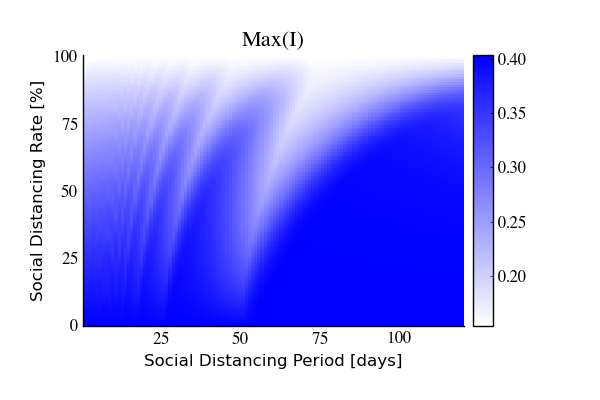
\includegraphics[width=0.49\textwidth]{epidemic-periodic-heatmap.png}
	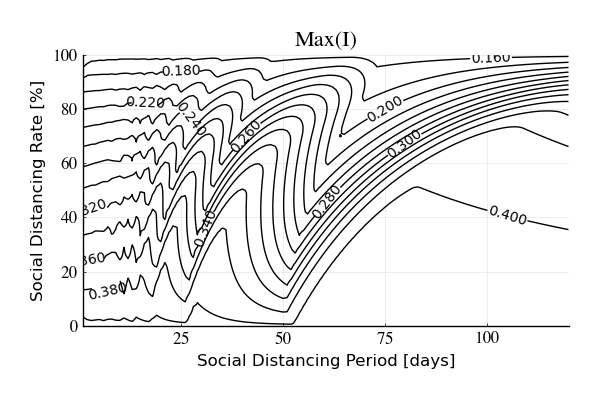
\includegraphics[width=0.49\textwidth]{epidemic-periodic-contour.png} 
\end{frame}

\begin{frame}{A similar pattern for a combination of a single interval SD and a periodic relaxation policy}
	Effect of periodic relaxation policy in combination with a single interval social distancing for \textit{SIR} model. The dashed orange lines represent the infected compartment peak time without the single interval social distancing policy. \\ \vspace{0.5cm}
	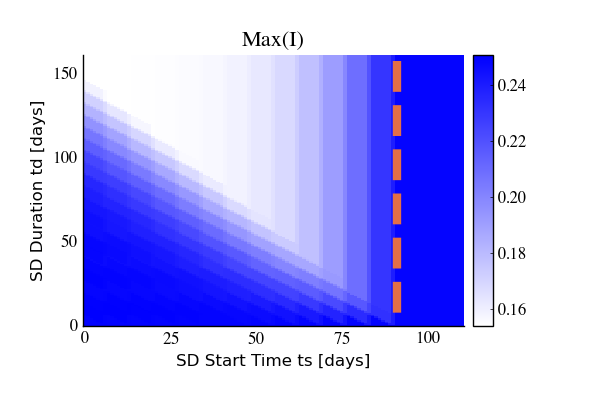
\includegraphics[width=0.49\textwidth]{epidemic-sp-heatmap1.png}
	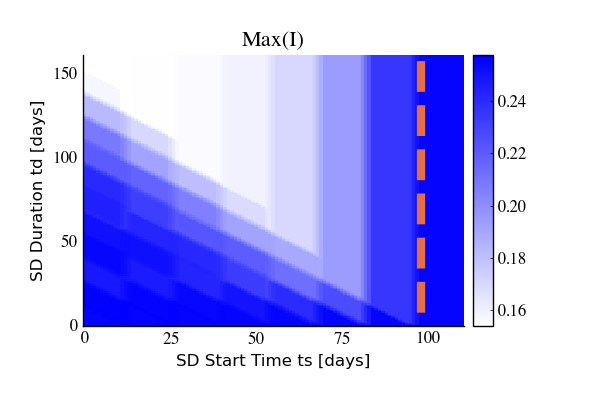
\includegraphics[width=0.49\textwidth]{epidemic-sp-heatmap2.png} 
\end{frame}

\subsection{Quasi steady state}
\begin{frame}{Modeling a prolonged outbreak}
	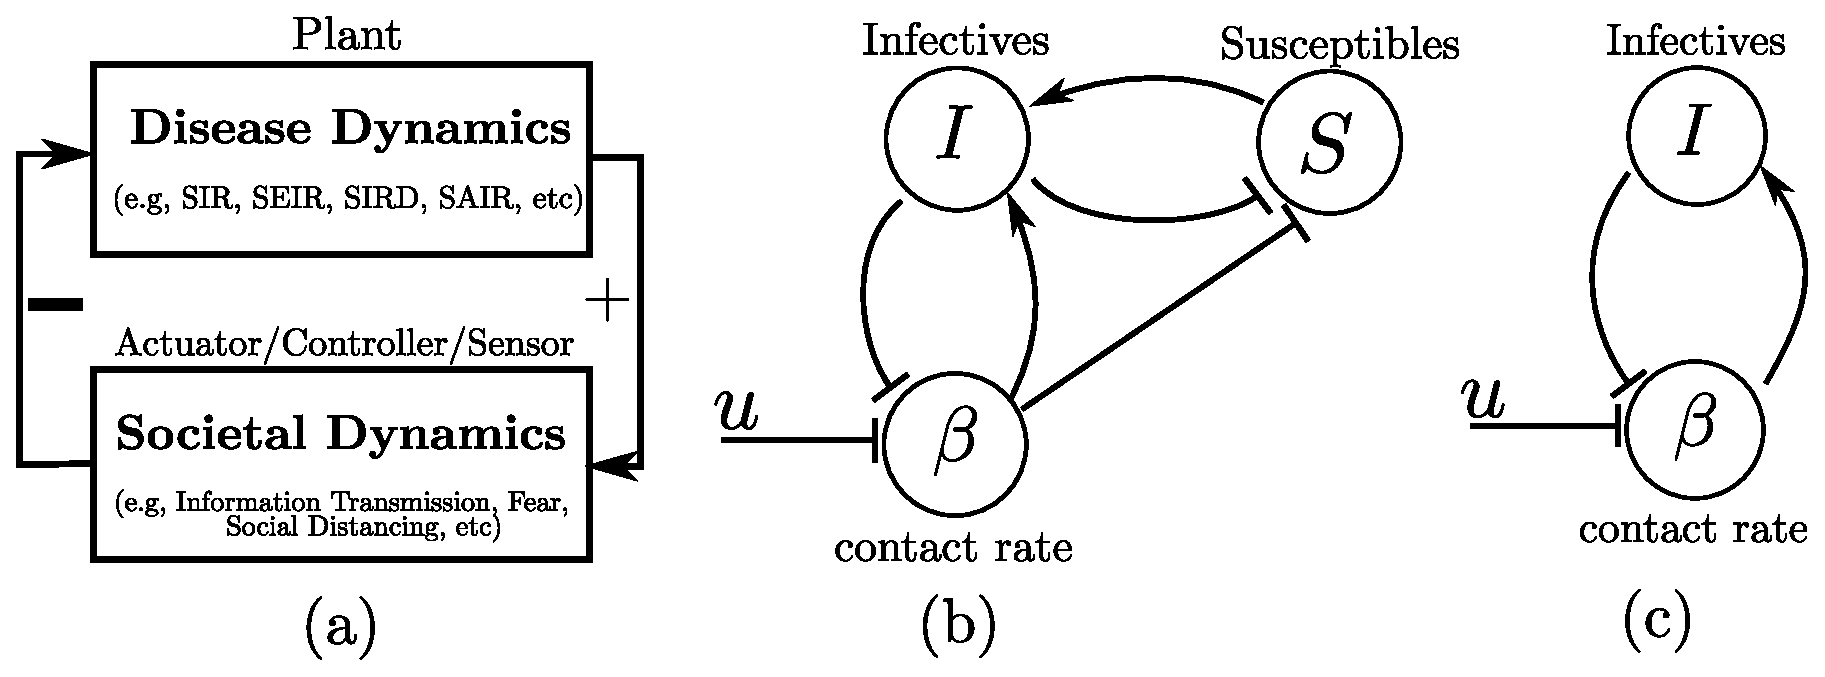
\includegraphics[width=1\textwidth]{epidemic-qss.eps} \\ \vspace{0.5cm}
	\small
	(a) Standard control theoretic framework for an epidemic model. (b) A minimal regulated SIR model, and (b) the reduced regulated SIR model in the case of a large population over short time periods (e.g., less than a year).
\end{frame}

\begin{frame}{Fitting to published data}
	An initial surge followed by a plateau during the summer 2020. \\ \vspace{0.5cm}
	This can be interpreted as a QSS in the proposed model. \\ \vspace{0.5cm}
	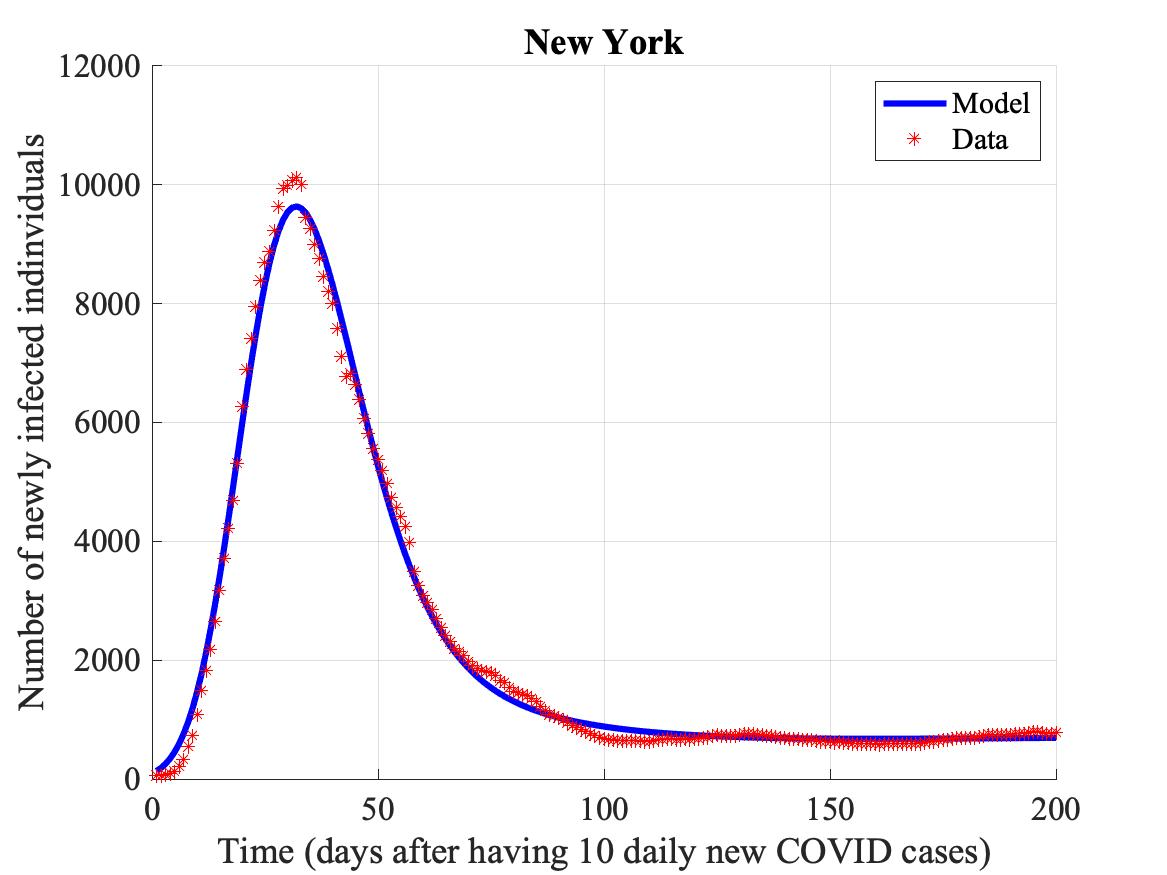
\includegraphics[width=0.49\textwidth]{epidemic-NewYork.jpeg} 
%	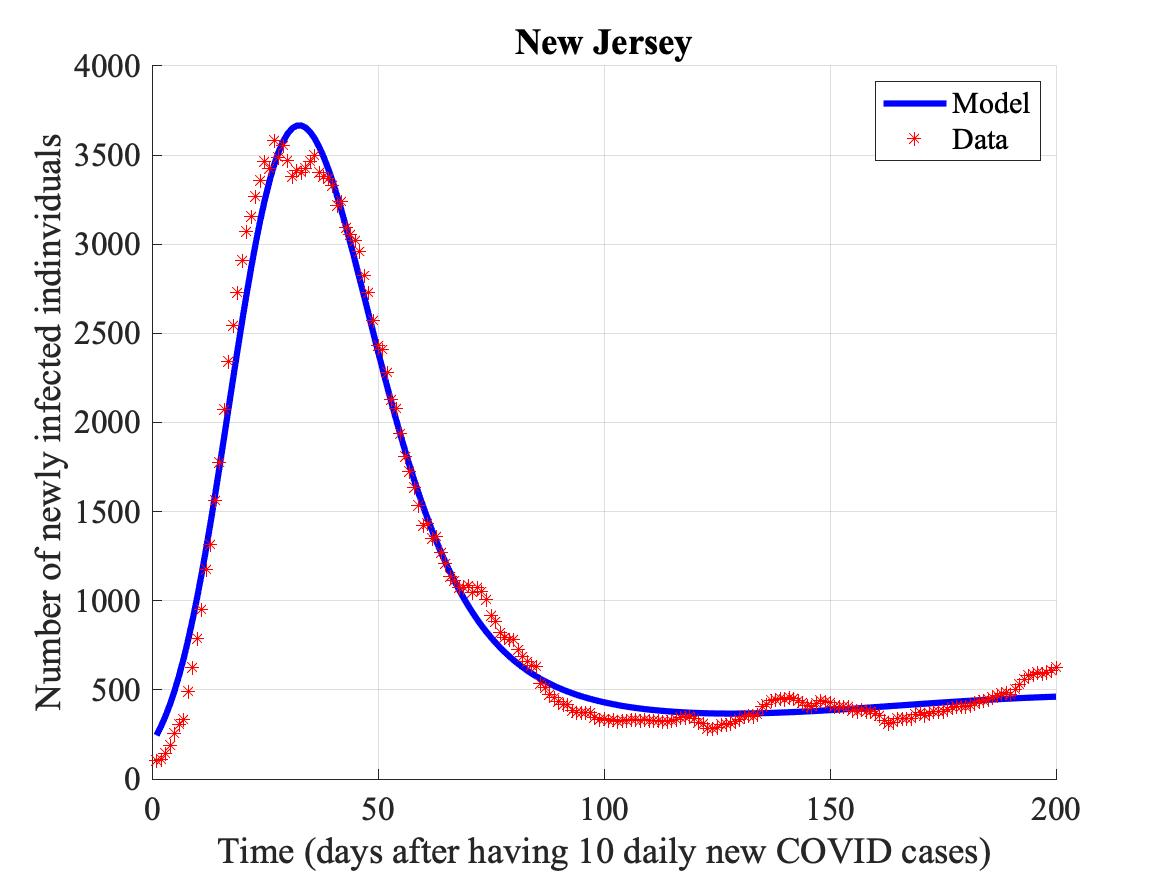
\includegraphics[width=0.32\textwidth]{epidemic-NewJersey.jpeg} 
	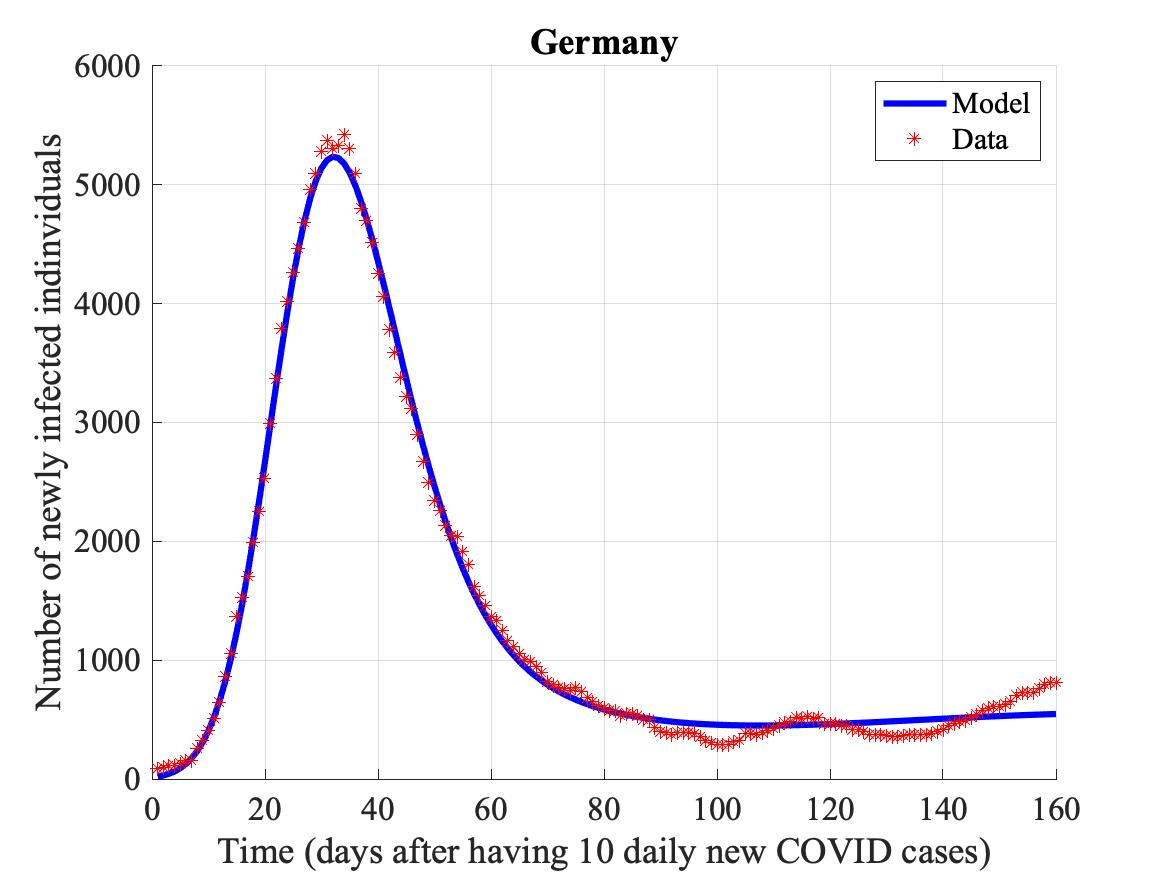
\includegraphics[width=0.49\textwidth]{epidemic-Germany.jpeg} 
\end{frame}
%-------------------------------------------------%
\section{Acknowledgment}

\begin{frame}{This work is a result of teamwork}
	\small \hspace{1cm}
	{\begin{tabular}{r@{}l}
			Advisor:   \  & Eduardo Sontag \\ 
			Lab members:   \  & M. Ali Alradhawi, Anh Phong Tran, Zheming An, \\ 
			&  William Cho, Shu Wang, Tianchi Chen. \\ \\
			Presented & \, projects  \\ \\
			Chemotherapy: \  & Anh Phong Tran, Irina Kareva, M. Ali Alradhawi, \\ 
			& and Waxman Lab.\\
			Epidemics: \ & James Greene, M. Ali Alradhawi. \\ \\
			Other & \, projects  \\ \\
			\scriptsize Immunotherapy: \ & Irina Kareva, Kumpal Madrasi, Abed Alnaif, \\ & Anup Zutshi, and EMD Serono Inc team. \\ 
			\scriptsize Parkinson's Disease: \ & AMP-PD research community, and Sanofi team.  \\ 
			Ribosome: \ & M. Ali Alradhawi, Michael Margaliot, Nikolai Slavov, \\ & Edward Emmott. \\ \\
			Open-source & \, community: Julia team, Gleb Pogudin, Esteban Vargas.  \\
			& Bioconductor project.  \\
		\end{tabular}
	}
\end{frame}

\end{document}